Os resultados alcançados abrangem diversas áreas do projeto, evidenciando o progresso em múltiplas frentes. Entre os principais destaques, estão a prototipação da aplicação móvel e web, o desenvolvimento da aplicação web, e a modelagem do banco de dados não relacional, contemplando os modelos conceitual, lógico e físico. Também foram elaborados os diagramas de casos de uso, classes e objetos, além da construção do modelo de negócios Canvas. Para a organização e gestão do projeto, a equipe adotou a ferramenta Figma, que, por meio da extensão FigJam, possibilitou a aplicação prática da metodologia Kanban. Essa extensão também desempenhou o papel de repositório central, reunindo e disponibilizando todos os elementos mencionados para consulta e análise colaborativa da equipe.

\subsection*{Protótipo do Sistema}

A \Cref{fig:ux-mobile01} representa a interface inicial da aplicação destinada a dispositivos móveis. Após a verificação bem-sucedida dos dados fornecidos no login, os usuários serão redirecionados para esta tela principal. Nesta interface, os usuários terão à disposição o pré-cadastro individual de cada bubalino. Nessa seção, o usuário é encarregado de manipular dados essenciais, tais como nome, identificação (número de identificação da tag), data de nascimento, peso em kg, sexo, raça, e a adição de uma foto para aprimorar a identificação do animal.

\newpage
\begin{figure}[!h]
\centering
\caption{Tela Inicial}%
\label{fig:ux-mobile01}
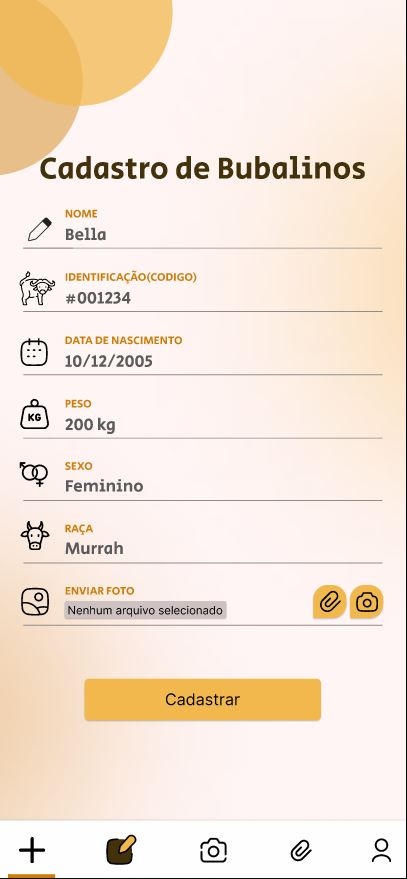
\includegraphics[scale=0.5]{Illustrations/UX-Mobile/Mobi-02.JPG}
\SourceOrNote{Autoria Própria (2024)}
\end{figure}

Após a conclusão do cadastro do bubalino, os usuários têm a opção de visualizar um prontuário abrangente de todos os animais cadastrados, conforme mostrado na \Cref{fig:ux-mobile02}. Este prontuário oferece informações detalhadas, incluindo nome, número de identificação da tag, sexo, raça. Caso o usuário queira ter uma visão mais detalhada de um prontuário, ele pode acessá-lo pelo segundo ícone no canto superior direito do prontuário .

\newpage
\begin{figure}[!h]
\centering
\caption{Tela Prontruarios}%
\label{fig:ux-mobile02}
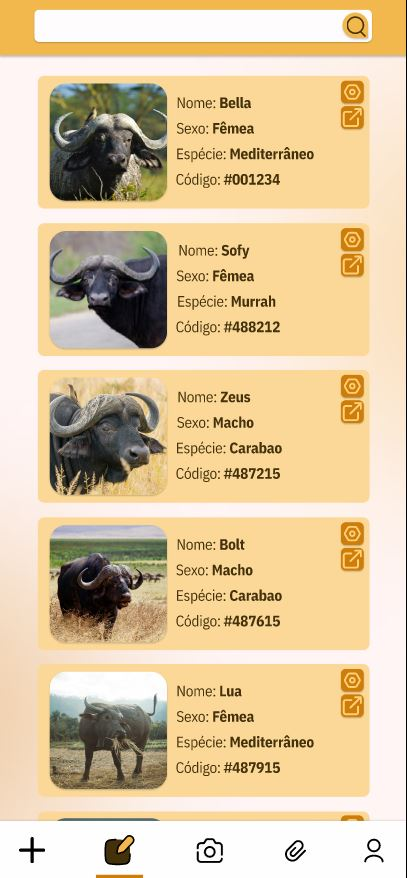
\includegraphics[scale=0.5]{Illustrations/UX-Mobile/Mobi-03.JPG}
\SourceOrNote{Autoria Própria (2024)}
\end{figure}

Caso o funcionário escolha o ícone mencionado anteriormente, ele será redirecionado para uma nova tela \Cref{fig:ux-mobile03} onde poderá visualizar e cadastrar novos dados do búfalo escolhido. Nesta tela, é possível inserir e atualizar informações zootécnicas, como peso, altura e alimentação, além de dados sanitários, como vacinas e tratamentos realizados. No caso de uma búfala, também é possível registrar dados reprodutivos, como ciclos de cio, inseminações e partos. Esta funcionalidade visa proporcionar um controle mais completo e preciso sobre a saúde e o desempenho dos animais, facilitando a gestão e melhorando o bem-estar dos bubalinos.

\newpage
\begin{figure}[!h]
\centering
\caption{Tela Prontruario Específico}%
\label{fig:ux-mobile03}
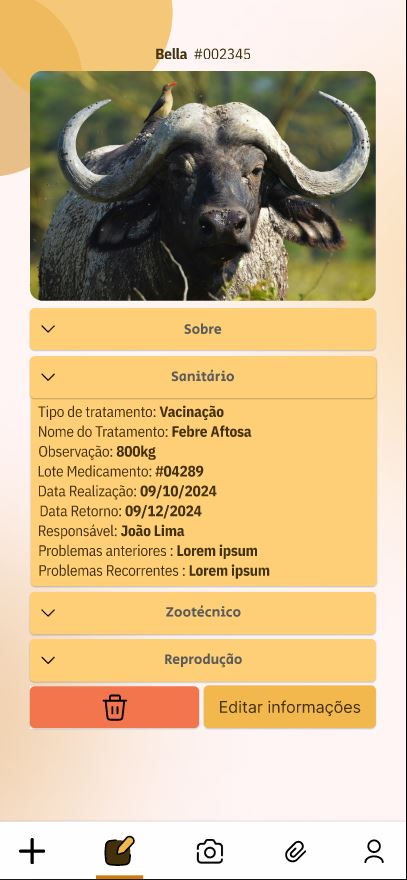
\includegraphics[scale=0.4]{Illustrations/UX-Mobile/Mobi-03.02.JPG}
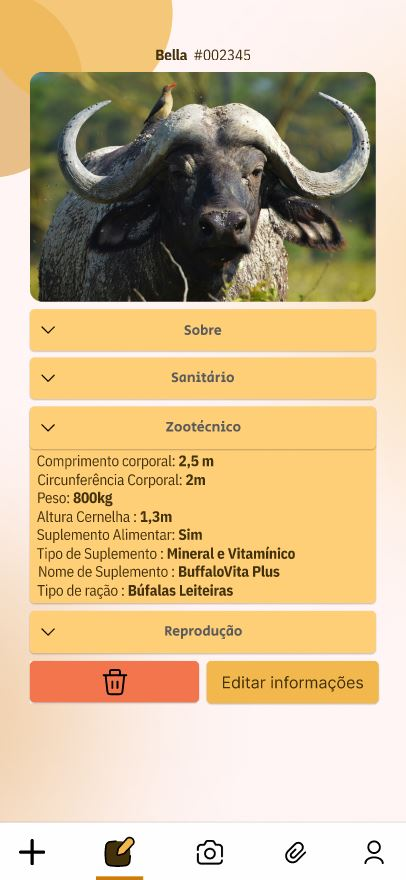
\includegraphics[scale=0.4]{Illustrations/UX-Mobile/Mobi-03.03.JPG}
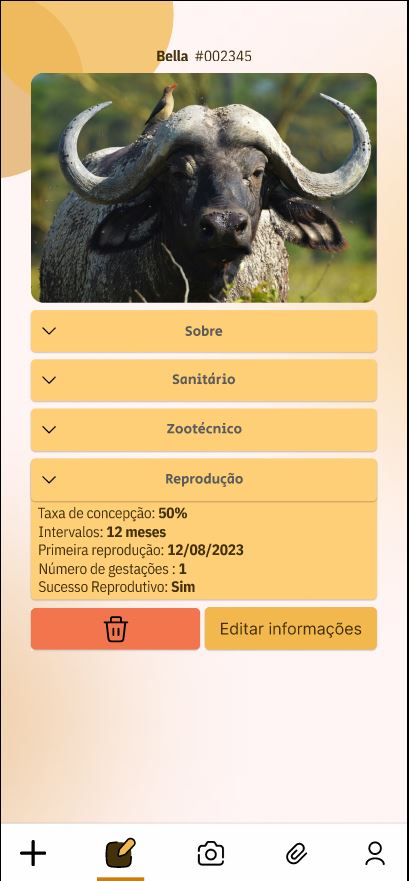
\includegraphics[scale=0.4]{Illustrations/UX-Mobile/Mobi-03.04.JPG}
\SourceOrNote{Autoria Própria (2024)}
\end{figure}

Na aplicação para dispositivos móveis, também há uma ferramenta que utiliza a metodologia de Kanban \Cref{fig:ux-mobile04} para melhorar a agilidade no manejo dos bubalinos. Essa ferramenta ajuda os funcionários a visualizar as demandas que o proprietário deseja que sejam realizadas com os animais, como tratamentos específicos para determinadas raças, por exemplo. Assim, é possível ter um controle claro do que precisa ser feito, o que está em andamento, o que está parado e o que já foi concluído. Isso facilita a organização e a priorização das tarefas, garantindo um manejo mais eficiente e organizado dos bubalinos.

\newpage
\begin{figure}[!h]
\centering
\caption{Tela Demandas}%
\label{fig:ux-mobile04}
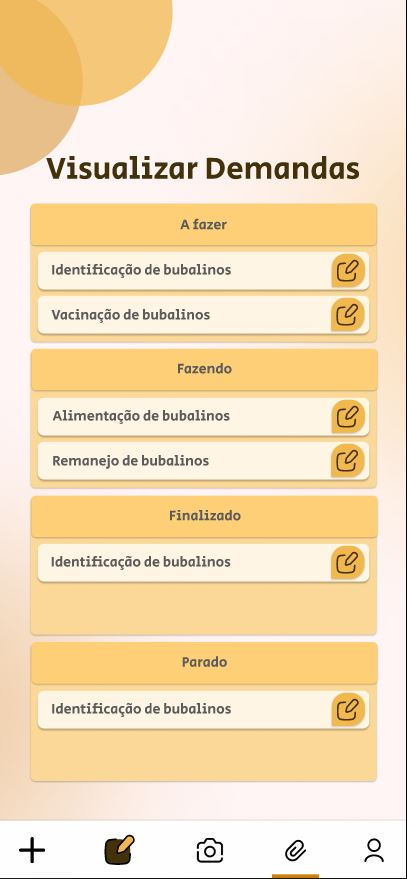
\includegraphics[scale=0.6]{Illustrations/UX-Mobile/Mobi-04.JPG}
\SourceOrNote{Autoria Própria (2024)}
\end{figure}

Para o sistema web, destinado ao proprietário do criadouro, foram prototipadas diversas telas. A tela inicial \Cref{fig:ux-pc01} apresenta informações essenciais para o gerenciamento do criadouro. Nela, o proprietário pode visualizar a quantidade de animais ativos, usuários ativos e inativos, além de gráficos que demonstram a taxa de natalidade, prenhez e gestação. Também são exibidos comparativos detalhados sobre as quantidades de cada raça e sexo, proporcionando uma visão ampla do rebanho. Por fim, a tela inclui um histórico das últimas tarefas realizadas no criadouro, garantindo maior controle e organização das atividades.

\newpage
\begin{figure}[!h]
\centering
\caption{Tela Inicial}%
\label{fig:ux-pc01}
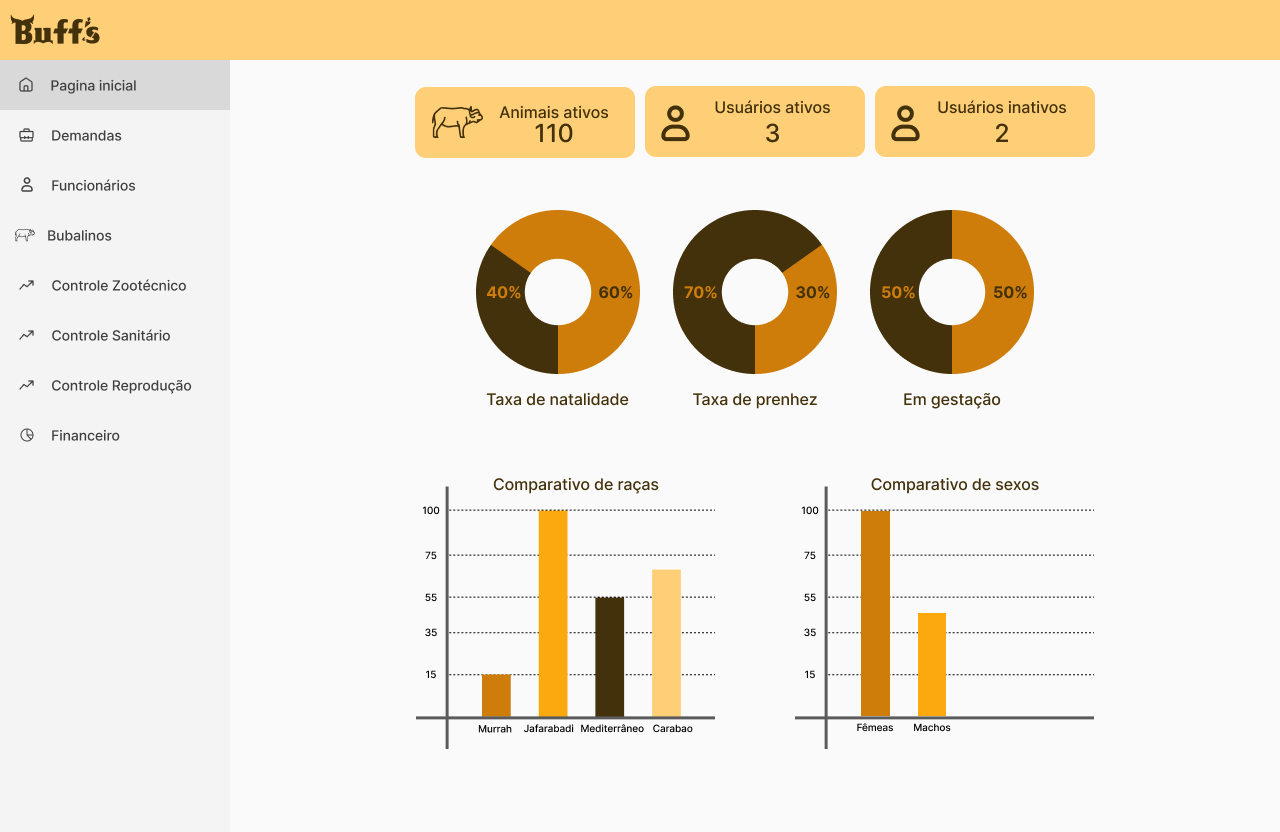
\includegraphics[scale=0.3]{Illustrations/UX-PC/Pc-01.png}
\SourceOrNote{Autoria Própria (2024)}
\end{figure}

Na tela subsequente \Cref{fig:ux-pc02}, o proprietário pode visualizar as demandas já atribuídas e verificar o status de cada uma delas, classificadas como "Em produção" ou "Finalizada". Além disso, é possível conferir detalhadamente quais demandas foram designadas a cada funcionário e, caso necessário, atribuir novas tarefas. Essa funcionalidade permite ao proprietário manter o controle sobre as atividades em andamento, garantindo uma gestão mais eficiente e organizada do criadouro.

\begin{figure}[!h]
\centering
\caption{Tela Atribuição de demandas}%
\label{fig:ux-pc02}
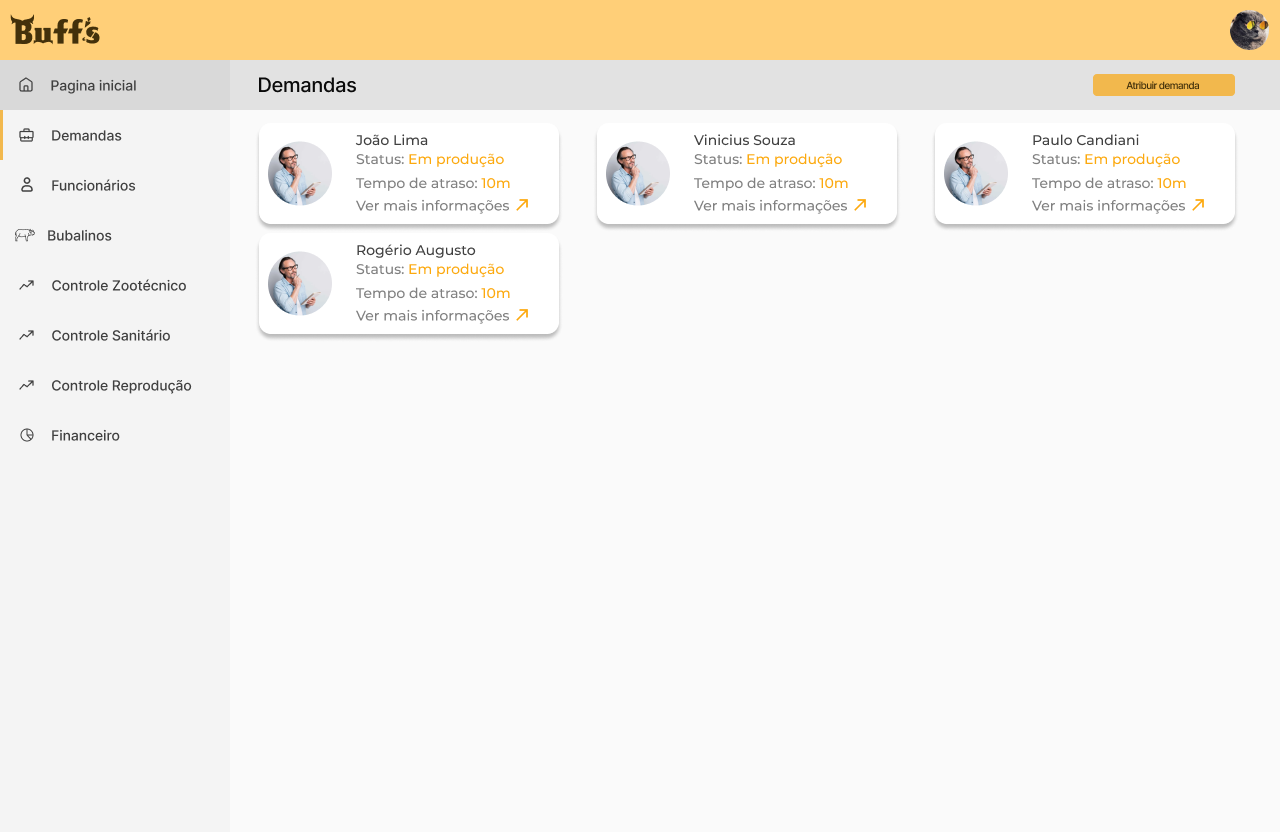
\includegraphics[scale=0.3]{Illustrations/UX-PC/Pc-02.png}
\SourceOrNote{Autoria Própria (2024)}
\end{figure}

O proprietário possui também uma tela dedicada ao cadastro de funcionários \Cref{fig:ux-pc03}, onde ele pode adicionar novos membros da equipe e atribuir-lhes credenciais de acesso à aplicação móvel. Essa funcionalidade garante que apenas funcionários autorizados tenham permissão para utilizar a plataforma móvel, mantendo a segurança e a integridade dos dados do criadouro.

\begin{figure}[!h]
\centering
\caption{Tela Cadastro de funcionarios}%
\label{fig:ux-pc03}
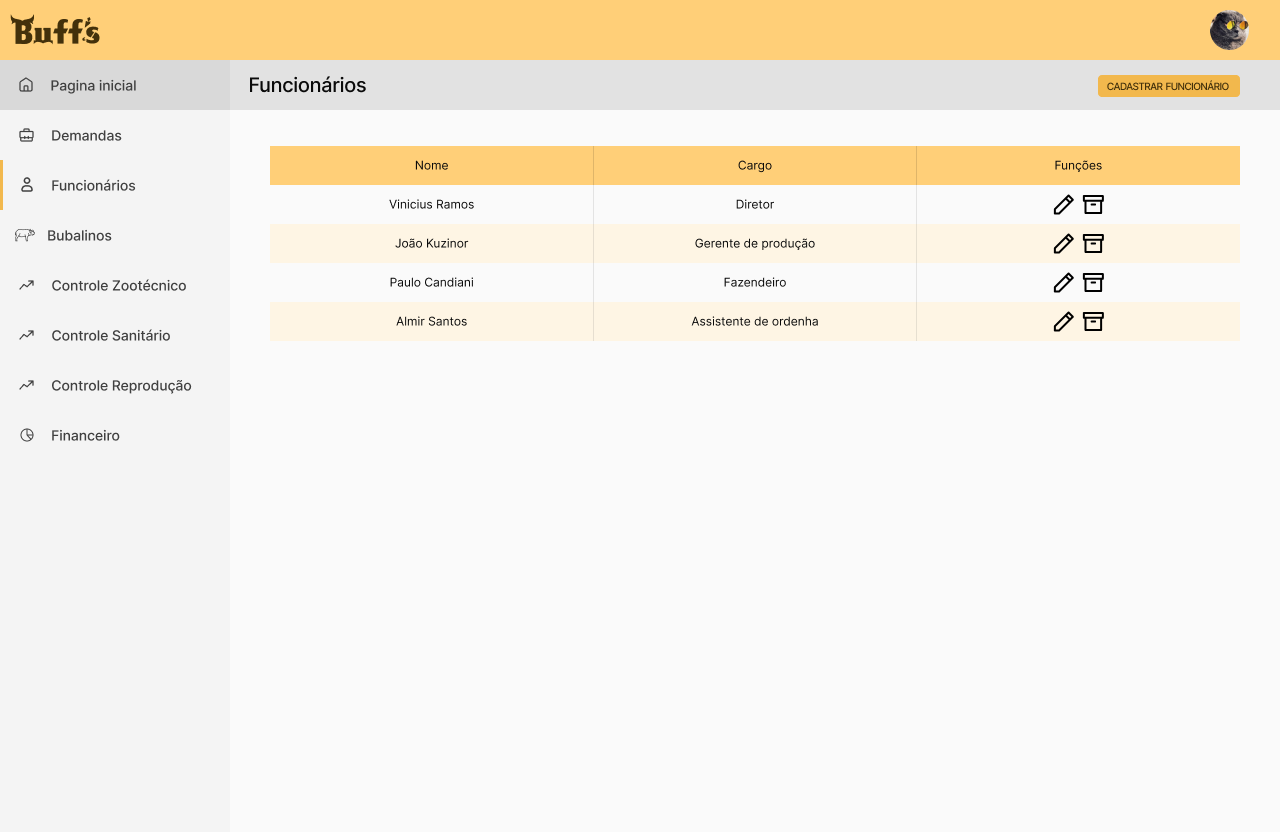
\includegraphics[scale=0.3]{Illustrations/UX-PC/Pc-03.png}
\SourceOrNote{Autoria Própria (2024)}
\end{figure}

Para que o proprietário tenha uma visualização abrangente de seus bubalinos, foi desenvolvida a tela "Bubalinos" \Cref{fig:ux-pc04}, onde todos os animais do criadouro são listados em uma tabela. Nessa interface, é possível acessar informações zootécnicas e sanitárias detalhadas de cada animal, facilitando o acompanhamento e a gestão eficiente do rebanho.

\newpage
\begin{figure}[!h]
\centering
\caption{Tela Bubalinos}%
\label{fig:ux-pc04}
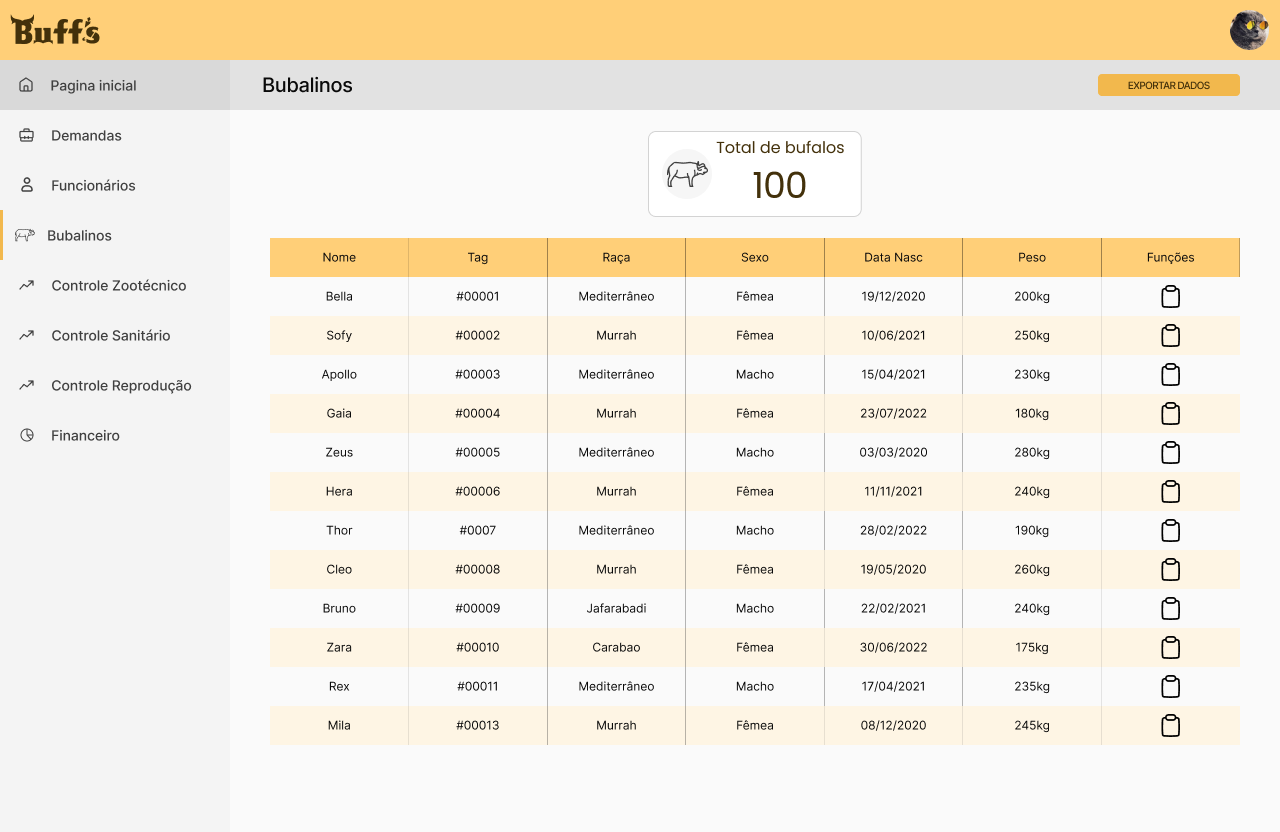
\includegraphics[scale=0.28]{Illustrations/UX-PC/Pc-04.png}
\SourceOrNote{Autoria Própria (2024)}
\end{figure}

Além disso, existem telas específicas destinadas a cada nicho, como a tela de "Dados Zootécnicos" \Cref{fig:ux-pc05} e a de "Dados Sanitários" \Cref{fig:ux-pc06} Cref de cada bubalino. Essas interfaces permitem ao proprietário acessar e gerenciar informações detalhadas relacionadas ao desempenho produtivo, histórico reprodutivo e condições de saúde de cada animal, apresentando gráficos para uma visualização mais clara e tabelas organizadas para consulta dos dados de forma estruturada e acessível.

\begin{figure}[!h]
\centering
\caption{Controle Zootecnico}%
\label{fig:ux-pc05}
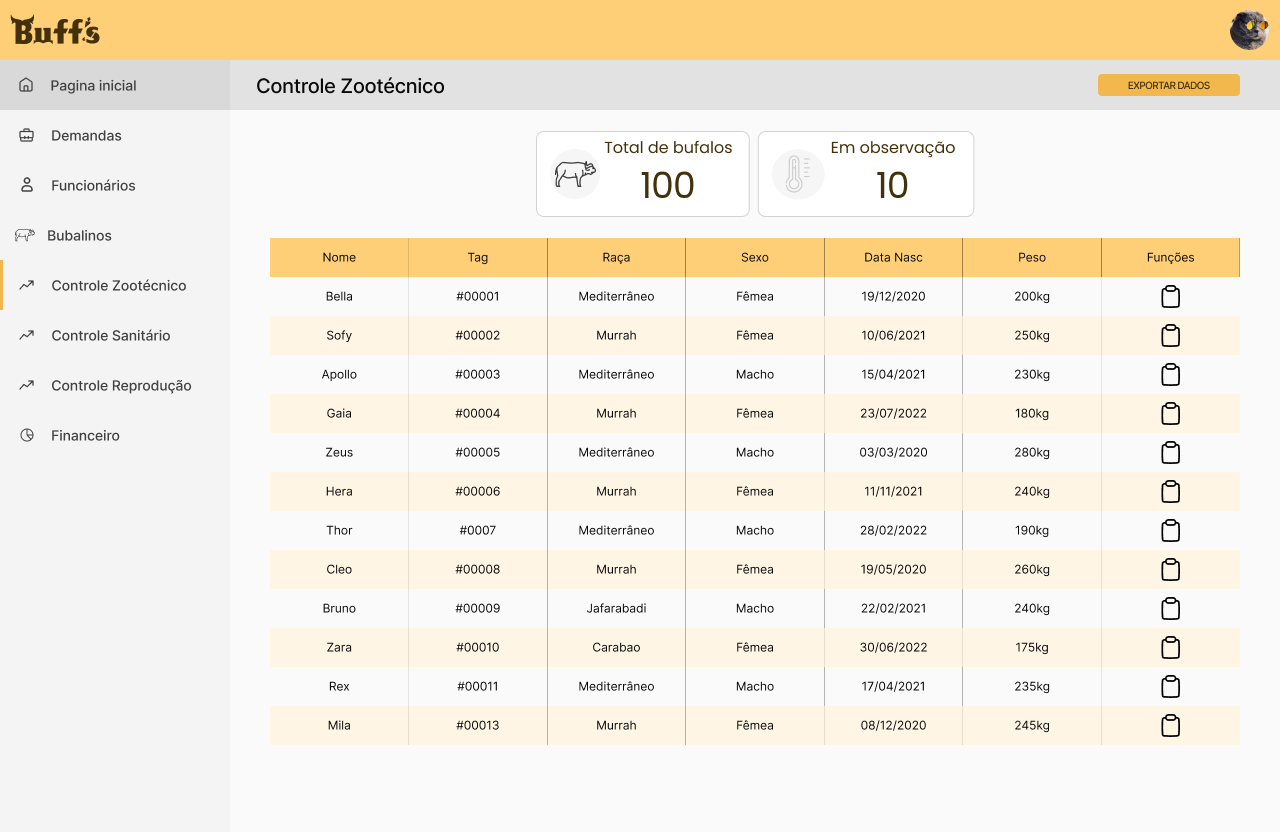
\includegraphics[scale=0.28]{Illustrations/UX-PC/Pc-05.png}
\SourceOrNote{Autoria Própria (2024)}
\end{figure}

\newpage
\begin{figure}[!h]
\centering
\caption{Controle Sanitario}%
\label{fig:ux-pc06}
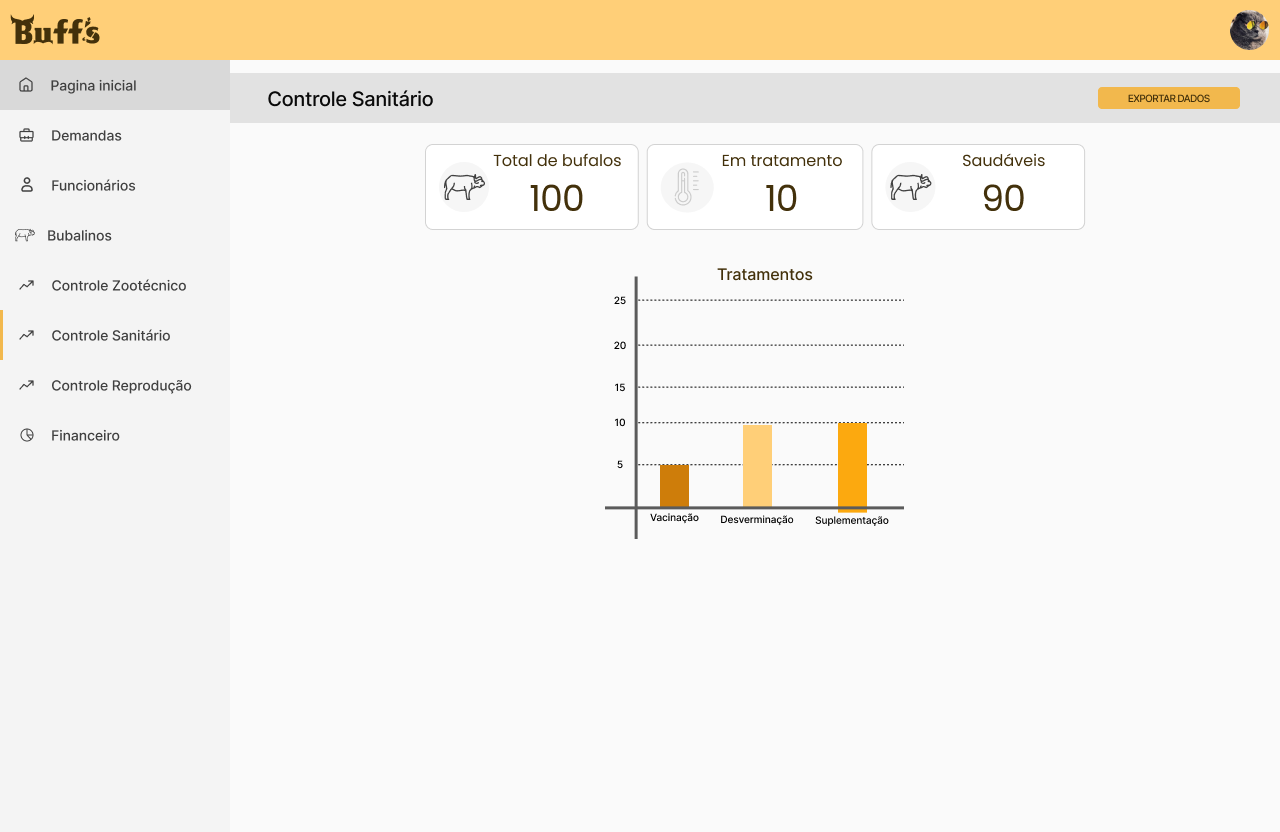
\includegraphics[scale=0.3]{Illustrations/UX-PC/Pc-06.png}
\SourceOrNote{Autoria Própria (2024)}
\end{figure}

\subsection*{Modelagem do Banco de Dados}

A representação gráfica da modelagem de Banco de Dados \Cref{fig:banco1} e \Cref{fig:banco2}  oferece uma visão perspicaz e abrangente da estrutura que será implementada no banco de dados não relacional (NoSql). Essa representação gráfica é fundamental, pois proporciona uma compreensão detalhada e clara de como os dados serão organizados, destacando as entidades, atributos e fornecendo uma visão intuitiva da arquitetura do sistema de armazenamento de informações. 

\begin{figure}[!h]
\centering
\caption{Modelo Conceitual}%
\label{fig:banco1}
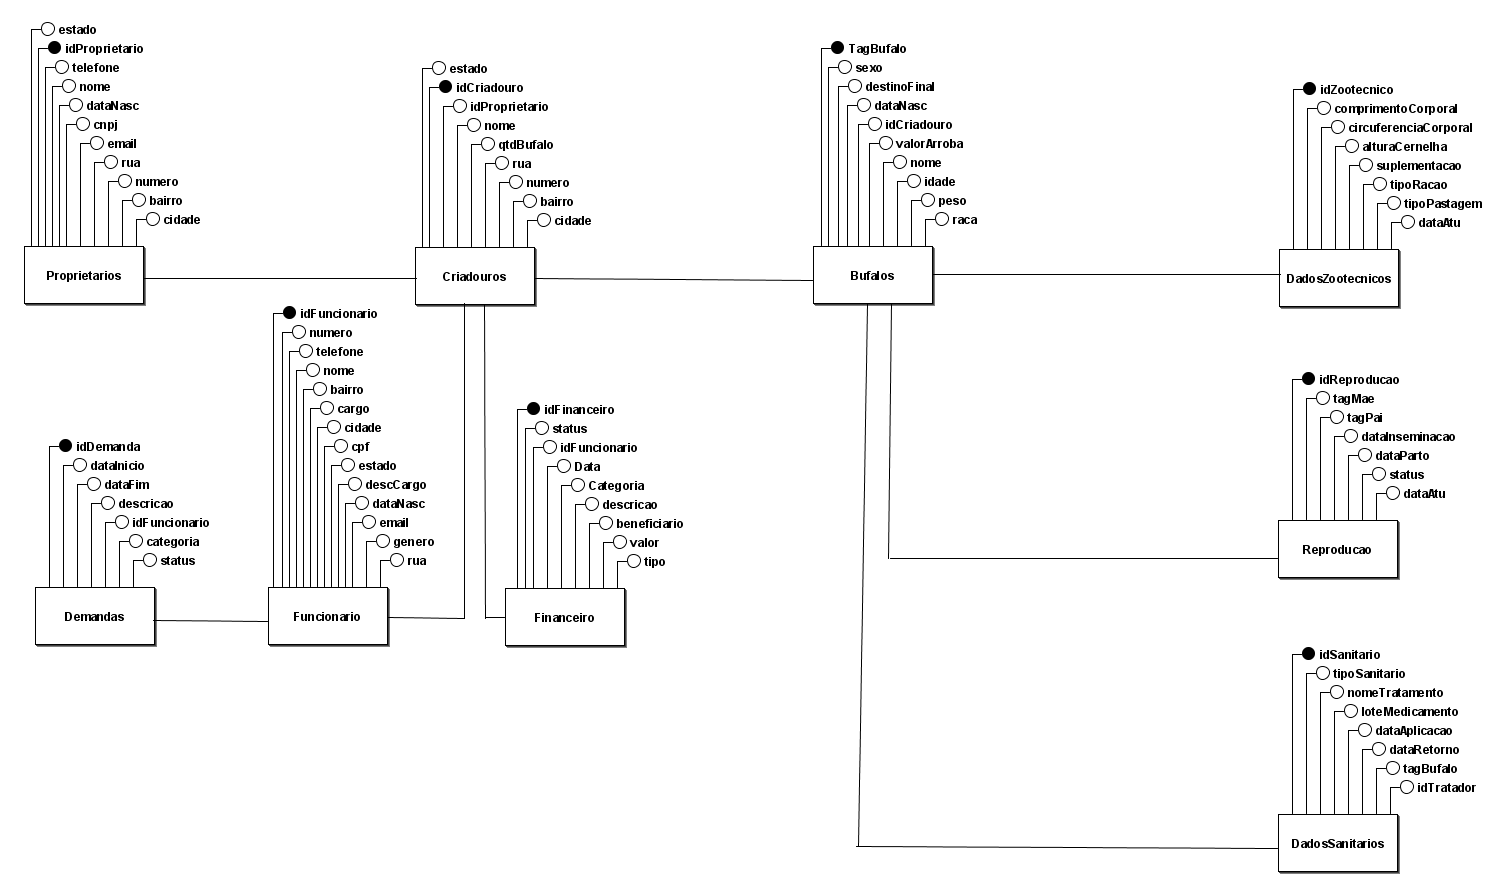
\includegraphics[scale=0.2]{Illustrations/Conceitual3Sem.png}
\SourceOrNote{Autoria Própria (2024)}
\end{figure}

\newpage

\begin{figure}[!h]
\centering
\caption{Modelo Logico}%
\label{fig:banco2}
\includegraphics[scale=0.2]{Illustrations/Lógico3Sem.png}
\SourceOrNote{Autoria Própria (2024)}
\end{figure}

Essa etapa é crucial para garantir que o sistema não apenas armazene dados, mas sim deixa claro a possibilidade de recuperar dados, mas também gerenciá-los de maneira eficiente e consistente, alinhada com a estrutura cuidadosamente planejada durante as fases de modelagem. A implementação bem-sucedida do banco de dados é fundamental para a funcionalidade global do sistema, promovendo a integridade e a eficácia na manipulação dos dados. Seguindo as etapas anteriores, concretizou-se o banco de dados físico.

\subsection*{Diagrama de Redes}

Para o sistema que abrange tanto desktop quanto dispositivos móveis, foi desenvolvido um diagrama \Cref{fig:redes} detalhado para ilustrar a estrutura de rede necessária. Este diagrama inclui componentes essenciais como o provedor de internet, o modem para conectar-se à internet, um switch para gerenciar a comunicação entre os dispositivos, um roteador Wi-Fi para fornecer conectividade sem fio, e, é claro, os próprios dispositivos, como computadores desktop e dispositivos móveis. Essa representação visual oferece uma visão abrangente da infraestrutura de rede, delineando como cada componente se conecta e interage para garantir uma comunicação eficiente e confiável em todo o sistema.

\newpage
\begin{figure}[!h]
\centering
\caption{Diagrama de Rede}%
\label{fig:redes}
\includegraphics[scale=0.04]{Illustrations/diagramaRedes.png}
\SourceOrNote{Autoria Própria (2024)}
\end{figure}

\subsection*{Diagramas UML}

A partir do Diagrama de Caso de Uso (DCU) \Cref{fcht:casodeuso}, é possível identificar o ator principal deste sistema, que é o usuário, abrangendo tanto os proprietários quanto os funcionários. Realiza-se, então, o mapeamento das ações do usuário identificado. Essas ações abrangem desde a criação da conta, na Dashboard, para o acesso à aplicação em dispositivos móveis. Esse mapeamento detalhado proporciona uma compreensão abrangente das interações do usuário com o sistema.


\begin{flowchart}[!htb]
\centering
\caption{Diagrama Casos de Uso}%
\label{fcht:casodeuso}
\includegraphics[scale=0.04]{Illustrations/casosUso.png}
\SourceOrNote{Autoria Própria (2024)}
\end{flowchart}
\newpage

Além disso, foi elaborado o diagrama de classes \Cref{fcht:classe}, uma etapa fundamental no desenvolvimento do sistema, pois permite uma representação visual das entidades e suas interações, contribuindo para a definição clara das classes e suas respectivas funções. Essa ferramenta desempenha um papel crucial na arquitetura e organização do código, facilitando o entendimento e a manutenção do sistema ao longo do tempo.

\begin{flowchart}[!htb]
\centering
\caption{Diagrama de classe}%
\label{fcht:classe}
\includegraphics[scale=0.04]{Illustrations/casosClasse.png}
\SourceOrNote{Autoria Própria (2024)}
\end{flowchart}

E por último, foi elaborado o diagrama de objetos \Cref{fcht:obejto}, uma etapa essencial para exemplificar quais dados devem ser inseridos em cada atributo das instâncias de classe. Esse diagrama proporciona uma visão detalhada das relações entre os objetos e seus atributos, facilitando a compreensão do fluxo de dados dentro do sistema

\begin{flowchart}[!htb]
\centering
\caption{Diagrama de objeto}%
\label{fcht:obejto}
\includegraphics[scale=0.04]{Illustrations/casosObjeto.png}
\SourceOrNote{Autoria Própria (2024)}
\end{flowchart}

O Modelo de Negócios Canvas \Cref{fig:canvas}, propõe agilizar o processo de manejo de bubalinos como sua principal proposta de valor. Este projeto tem como objetivo atender pecuaristas com foco na criação de bubalinos, estabelecendo parcerias com fornecedores de equipamentos agropecuários, universidades e instituições de pesquisa para inovação tecnológica, além da colaboração com associações de produtores de bubalinos.

\begin{figure}[!h]
\centering
\caption{Canvas}%
\label{fig:canvas}
\includegraphics[scale=0.06]{Illustrations/canvas.png}
\SourceOrNote{Autoria Própria (2024)}
\end{figure}

Os canais de comunicação estabelecidos abrangem vendas diretas para fazendas, plataformas online, comunicação por telefone e email.
Para a construção da aplicação móvel, identificaram-se recursos necessários, como a disponibilidade de equipamentos e a configuração de um banco de dados. As principais despesas previstas para a execução do projeto incluem a contratação da equipe de desenvolvimento e a aquisição do ambiente para o desenvolvimento.
A fim de cobrir os custos do projeto, elaborou-se um esquema de serviços de suporte técnico e taxas de licenciamento do software como fontes de renda.

\subsection*{KanBam}


A metodologia "\textit{Kanban}" \Cref{fig:kanbam} desempenhou um papel fundamental na organização da equipe durante o desenvolvimento do trabalho. A estrutura foi dividida em quatro quadros principais: 'To do' (A fazer), 'In Progress' (Em andamento), 'Stopped' (Parado) e 'Done' (Concluído). Cada quadro teve uma função específica no gerenciamento do projeto. No quadro 'To do', eram agrupadas as tarefas ainda não iniciadas. O quadro 'In Progress' reunia as atividades que estavam sendo desenvolvidas, enquanto o quadro 'Stopped' indicava as tarefas que, por algum motivo, estavam pausadas temporariamente. Por fim, o quadro 'Done' registrava as tarefas já concluídas. Essa metodologia proporcionou à equipe uma visão ampla e organizada do andamento do projeto, facilitando o acompanhamento do progresso, a identificação de gargalos e a eficiência na execução das atividades.

\begin{figure}[!h]
\centering
\caption{KanBan}%
\label{fig:kanbam}
\includegraphics[scale=0.08]{Illustrations/KanBan.png}
\SourceOrNote{Autoria Própria (2024)}
\end{figure}

A visualização do processo por meio do "\textit{Kanban}" ilustra de maneira inequívoca a eficácia dessa abordagem organizacional. Ao utilizar essa plataforma, a equipe não apenas obteve uma visão abrangente das atividades em curso, mas também adotou uma maneira intuitiva de priorizar, rastrear e validar tarefas. A estruturação dos quadros não apenas otimizou a produtividade, mas também fomentou a comunicação transparente e a tomada de decisões informadas dentro da equipe.